\section{系统开发流程}

    按照现有嵌入式企业的嵌入式软件开发流程,开发一个嵌入式系统主要分为以下几个步骤。

\subsection{用户需求分析}

    根据现有的各种企事业单位对于考勤打卡的需求,需求的特性主要为特征性识别以及日志记录。
    
    因此,在总体设计上我计划采用最简单的由指纹识别模块获取输入,经过 MCU 中简单处理再转发给
    linux 下的控制主机的设计。

\subsection{嵌入式开发环境的搭建与说明}

    由于嵌入式开发所基于的 MCU 一般性能相当有限,就算是采用一般 linux 操作系统进行本机编译,其占用时间也会相对比较长,同时,也无法应对一些占用系统内存资源较大的编译场景。
    因此,在嵌入式开发中,一般通过交叉编译的方式实现在 x86\_64-linux 平台或其他通用操作系统架构平台上实现对于目标平台代码的编译以更好的利用硬件资源。

    在本文的实现过程中基于 \href{https://nixos.org/}{Nix} 管理 x86\_64-linux 平台实现了对 aarch64-unknown-linux 目标平台的编译,其中主要的编译工具链的部分直接采用原有 \href{https://github.com/rcore-os/arceos}{ArceOS} 操作系统实现的 Rust 语言交叉编译以及镜像处理步骤,将 Cargo 包管理工具直接生成的裸机 elf 文件通过 rust-objcopy 去除其中一些无关的信息,如调试信息等内容成为一个纯粹的二进制文件。 
  
    一般树莓派的流程由 保存在 Soc ROM 区中的 booloader 完成 SD 卡上 FAT32 分区的挂载以及加载第二阶段 bootcode.bin,但是由于我使用的树莓派4B (bcm2711) 相对于前代有不少的硬件更新,在我使用的树莓派中对应初始化,启用 GPU fireware 加载 start.elf 的 bootloader 代码都被实现在 EEPROM 中,以提升 ROM 代码的容错性。 
    在运行 start4.elf 文件时,其会对 sd 卡中的 config.txt 文件进行解析,完成对应如串口传输频率,是否启用 JTAG 调试等配置,还会将其中声明的镜像文件加载到内核地址,使 CPU 由 stand-by 状态开始执行内核初始化代码。

    在我开发的过程中参照 \href{https://github.com/rust-embedded/rust-raspberrypi-OS-tutorials}{rust-raspberrypi-OS-tutorials} 的串口传输工具完成了串口传输的配置。其中通过实现一个最小配置内核,实现了初始化对应端口(PIN 14,15)的替代方法声明以启动对应端口的传输声明。同时通过CH304 USB 转 TTL 串口传输模块发送开始传输信号给开发机中 Ruby 运行的应用程序,应用程序将内核镜像文件通过串口传输到树莓派4B内存中以完成镜像加载。最终最小配置内核将控权转交给内核镜像文件。

    \subsubsection{基于 Nix 构建可重构开发环境}

    作为一个标准开发操作系统的开发环境,必然是需要在同组内保持一定程度上的可重构性,易重构性以及同步性。基于这几种考量,我选用了 \href{https://nixos.org/}{Nix} flakes 对于项目整体依赖进行管理。就目前来看,除了对于使用到其他项目中的 docker 的部分,由于在 Non-NixOS 中,Nix 无法介入 systemctl 的管理而存在一定的不一致情况以及由于 WSL 对于串口设备连接的限制\footnote{在WSL中连接串口设备的时候,需要额外安装 usbipd},其他的部分表现良好,均能很好的在 WSL, NixOS, Debian 等常用开发系统中构建一致,可用的开发环境。

    % 具体在实现过程中,我通过 flakes.inputs 固定了后面引用的 Nixpkgs, rust-overlays 库。
    % 同时,使用 overlays 在原先 nixpkgs 上掩盖了我自己的派生以保证开发环境构建的一致性。
    % 在代码段\ref{nix-flake-overlays} 第 7-10 行实现了对于 rust nightly toolchain 的固定,
    % 在后文 11-17 行实现了对于 nixpkgs 特定版本 qemu 的选择,在 18-21 行实现了对于联网获取的编译工具链的固定。
    
    \begin{lstlisting}[language=nix
        , caption=my flakes
        , label = {nix-flake-overlays}
        , numbers = left
        , breaklines=true
        , breakatwhitespace=true]
overlays = [ 
    (import rust-overlay)
    (self: super: {
        rust-toolchain =
        let rust = super.rust-bin; in
            # The rust-toolchain when i make this file, which maybe change
            (rust.nightly."2020-04-07".override {
            extensions = [ "rust-src" "llvm-tools-preview" "rustfmt" "clippy" ];
            targets = [ "x86_64-unknown-none" "riscv64gc-unknown-none-elf" "aarch64-unknown-none-softfloat" ];
            });
        qemu7 = self.callPackage "${nixpkgs-qemu7}/pkgs/applications/virtualization/qemu" {
        inherit (self.darwin.apple_sdk.frameworks) CoreServices Cocoa Hypervisor;
        inherit (self.darwin.stubs) rez setfile;
        inherit (self.darwin) sigtool;
        # Reduces the number of qemu source files from ~10000 to ~3619 source files.
        hostCpuTargets = ["riscv64-softmmu" "riscv32-softmmu" "x86_64-softmmu" "aarch64-softmmu" ];
        };
        x86_64-linux-musl-cross = fetchTarball {
        url = "https://musl.cc/x86_64-linux-musl-cross.tgz";
        sha256 = "172zrq1y4pbb2rpcw3swkvmi95bsqq1z6hfqvkyd9wrzv6rwm9jw";
        };
    })
    \end{lstlisting}

    同时,为了保证引入的工具链能完整的运行,我根据 \href{}{nixpkgs} 中提出的 issue,对于部分存在的问题进行了修复。

    \begin{lstlisting}[language=nix
        , caption=flakes 特殊适配
        , numbers = left
        , breaklines=true
        , breakatwhitespace=true]
unset OBJCOPY # Avoiding Overlay
export LIBCLANG_PATH="${pkgs.llvmPackages.libclang.lib}/lib" # nixpkgs@52447
export LD_LIBRARY_PATH="${pkgs.zlib}/lib:$LD_LIBRARY_PATH" # nixpkgs@92946

export PATH=$PATH:${pkgs.aarch64-linux-musl-cross}/bin: # ... etc
    \end{lstlisting}

%     \newpage


\subsection{ArceOS 操作系统现有网络驱动实现分析}

    下图\ref{fig::cvitek}左侧的部分是 ArceOS 操作系统的整体布局,右侧是现有\href{https://github.com/yuoo655/arceos_net/tree/hsp}{cvitek 物理网卡驱动} 的逐层调用情况。

    该 cvitek 物理网卡驱动主要作用在华山派,荔枝派等主机上。但与我们采用的树莓派4B中由 Soc 中集成 MAC 实现不一样,他们采用的这款设备提供了一个额外的以太网 MAC 控制器的 IP 核DWMAC 来完成 MAC 层的实现。

        
    \begin{figure}[ht]
        \centering
        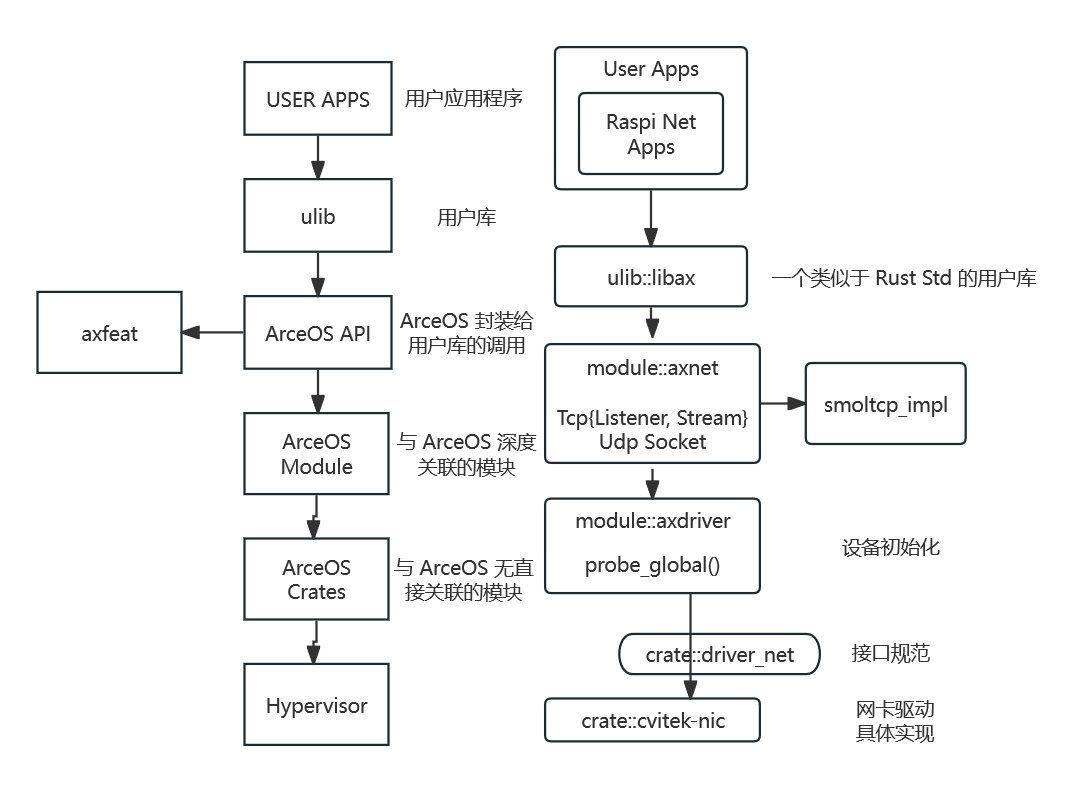
\includegraphics[scale=0.4]{imgs/cvitek.jpg}
        \caption{cvitek 驱动调用栈}    \label{fig::cvitek}
    \end{figure}

    在整套实现中,ulib::libax 通过调用 module::axnet 所实现的底层方法(如TcpSocket,UdpSocket等)实现了用于 TCP/UDP 通信的通信源语。
    在 module::axnet 中这个部分的实现是针对于 
    \href{https://github.com/smoltcp-rs/smoltcp}{smoltcp} 这个 tcp/ip 协议栈进行了针对性的改造(非标准库环境等改造)而完成的。
    如果在编译的时候添加了对应的 features, ArceOS 会自动根据 module::axdriver::build.rs 文件中所进行的声明,
    将一个带有不同设备名称的 feature 加入默认 feature list 中,以方便实现基于设备组(phy, net, block, display) 实现的自动驱动加载。
    在完成 build.rs 编译脚本中的检查等操作之后,Cargo 在对于 axdriver 进行编译的时候,
    就会识别到当前编译携带了 cvitekphy/nic feature 从而根据 \#[cfg(feature = "cvitekphy")] 启用 cvitek\_traits.rs 的编译。
    cvitek\_traits.rs 文件将 ArceOS 上层 module 所提供给下层 crates 的方法支持(如dma\_alloc\_pages,delay等)
    通过 traits 的默认实现传递给下方的 crates 进行使用以实现 crates 层逆向调用 modules 层方法的效果。
    \footnote{在cvitek\_traits.rs 文件中 CvitekPhyTraits 声明并实现于 CvitekPhyTraitsImpl }。
    同时,在 module::axnet::driver.rs 中基于 cfg\_if 库的条件编译语句也实现了将 cvitek 网卡驱动转换成为 AxNetDevice 
    并实现了 Driver traits 下属的 probe\_global 方法的效果。
    最后在 module::axdriver 中 for\_each\_driver 宏的帮助下,ArceOS 将各个加载的网卡驱动转换成为 
    Driver 并运行(probe\_global)初始化,并将其添加到 AllDevices 下属的结构体中。

    而根据 ArceOS 的规定,cvitek 以太网卡驱动的实际实现实际上被封装在各自的 crates 中。在 crates::driver\_net 包规定了一系列网络设备、
    所必须要实现的 traits(如 transmit, receive)等方法。
    新的网络驱动会使用其内部方法实现这些对应的 traits,将这些方法包装成为 ArceOS 的调用方法。

\subsection{以太网卡驱动实现}

    根据前文的分析,如果想要实现在 TRANSPORT 层或者 NETWORK 层实现树莓派和主机之间的通信效果,主要需要实现以太网 OSI 七层模型中的 DATA\_LINK 与 PHYDIVSL 层之间的通信,
    由下图\ref{fig::dataLink}可知,主要需要实现的部分在于使 Soc 上的 MAC 实现能通过 GMII, RGMII,Serial-GMII 等接口标准与 PHY 芯片进行联通,进而调用 PHY 芯片上对于以太网传输介质上光,电等信号进行解析的方法。
        
    \begin{figure}[ht]
        \centering
        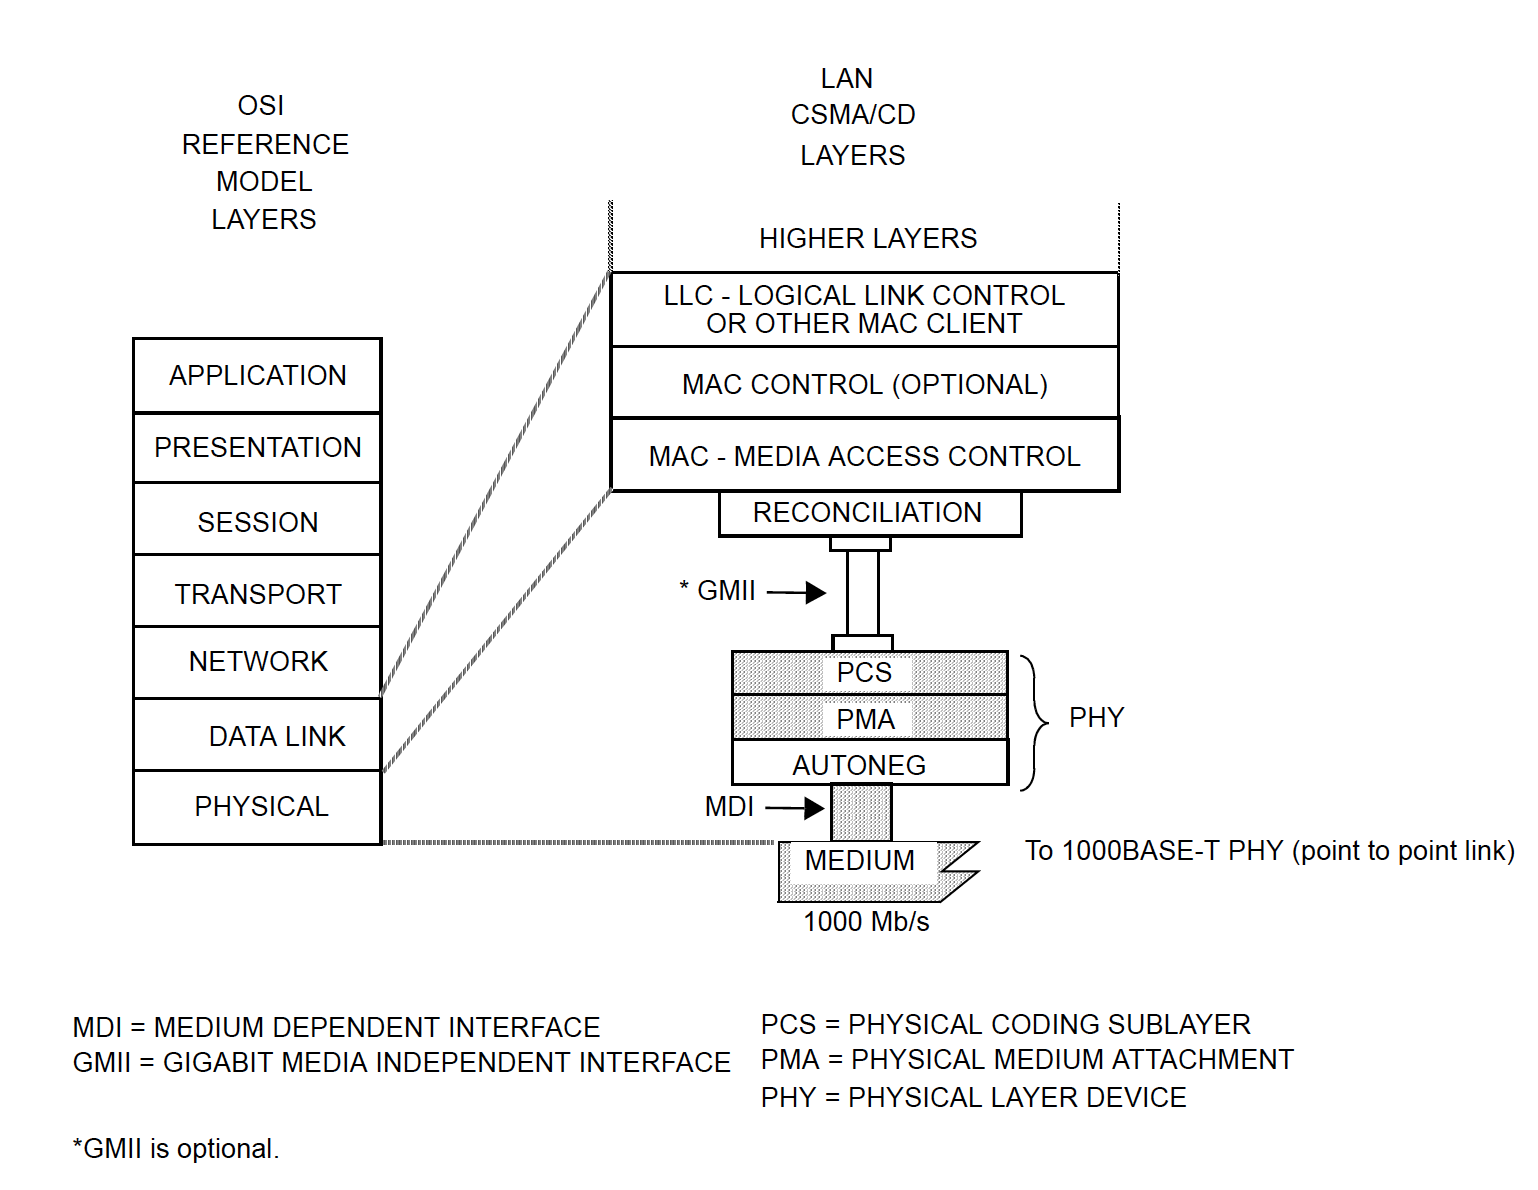
\includegraphics[scale=0.4]{imgs/data_link_layers.jpg}
        \caption{IEEE 802.8 数据链路层}    \label{fig::dataLink}
    \end{figure}

    基于 树莓派 4B Soc bcm2711 芯片手册,其板载 PHY 芯片 BCM54213PE 数据表以及 IEEE 802.3 协议手册可以了解到,目前 Soc 和 PHY 之间是存在直连的 RGMII 通信接口的。
    在 RGMII 通信接口中由 GTK\_CLK, RX\_CLK 实现双向时钟同步,TXD[0:3], RXD[0:3] 实现数据传输,TX\_CTL,RX\_CTL 实现数据传输控制,MDIO 和 MDC 实现 MAC 与 物理层的控制和状态关系的设置。
    \footnote{虽然在bcm2711数据手册GPIO替代函数表中有提到提供了 RGMII\_MDIO 与 RGMII\_MDC Pins,但是没有找到任何公开资料描述这个部分与底层之间是如何联系起来的}

    % TODO: 其中 GPIO 中也提供了一组 MDIO MDC 有点没太明白这段是为什么添加到这个地方?

    % \subsubsection{源码分析}

    根据对于 uboot 源码所进行的分析,在以太网 PHY 芯片中维持了如下的数据结构\ref{fig::uboot-genet-struct}。

    \begin{minipage}[t]{0.42\linewidth}
    \begin{lstlisting}[columns=fullflexible, label={fig::uboot-genet-struct}]       +
0x0    | IOBASE
+------|-----------------------------+
0x2000 | GENET_RX_OFF
       | [DMA_DESC_SIZE;TOTAL_DESCS]
0x2C00 | GENET_RDMA_REG_OFF
       | [DMA_RING_SIZE;DEFAULT_Q]
0x3000 | RDMA_RING_REG_BASE
       | [DMA_RING_SIZE]
0x3040 | RDMA_REG_BASE
       | dma_reg
+------|-----------------------------+
0x4000 | GENET_TX_OFF
       | As above ...
       +
        \end{lstlisting}
    \end{minipage}
    \quad
    \begin{minipage}[t]{0.5\linewidth}
        \vspace{2em}
        \setlength{\parindent}{1em}
        其中,IOBASE 为 BCM54213PE 芯片基于 MMIO 地址映射,在树莓派内存中对应的地址。
        在树莓派网卡中,0x2000-0x4000的地址主要分配给与Rx相关的结构体。0x4000-0x6000的地址分配给TX相关的结构体。

        这些结构体都是以太网卡中 DMA 模块至关重要的成分。
        以 0x2000 GENET\_RX\_OFF 开头,到 GENET\_RDMA\_REG\_OFF 为止的一段地址中保存了 256 个 DMA 描述符结构。
    \end{minipage}

    以 0x3000 GENET\_RDMA\_REG\_OFF 开头,到 RDMA\_RING\_REG\_BASE 为止的这一段地址中保存了 BCM54213PE 
    所支持的 16 个不同优先级别的接受环(方便 DMA 实现基于不同优先级的接受),
    还在 RDMA\_RING\_REG\_BASE 与 RDMA\_RING\_REG\_BASE 之间保存了一个默认的接受环。

    也就是说在 BCM54213PE 的硬件实现中提供了对于 16 个优先级队列,以及一个默认队列的支持。不过根据源代码,
    实际上不管是树莓派官方的 linux 内核或者 uboot 下的以太网驱动都没有全部使用这些队列。
    在树莓派中,将 256 个 DMA 描述符分配给五个队列,其中前四个队列分别占有 32 个描述符,第五个,也就是默认队列
    占有剩余的 128 个描述符。而在 uboot 中的实现考虑到了其需求,对于原先的设计进行了删减,
    直接将 256 个 DMA 描述符全部分给了默认队列(并没有使用优先级队列)。
    
    \begin{adjustwidth}{0cm}{} % NOTE: 消除全局段首锁紧带来的影响
    \begin{minipage}[b]{0.5\linewidth}
        \setlength{\parindent}{2em} % 段首缩进
        在 BCM54213PE DMA 模块中以太网模块初始化的过程中,会逐个将使用的 Rings 环进行初始化,
        每一个抽象意味上的环都是由 start\_addr 到 end\_addr 中的一段连续的 DMA 描述符组合而成的。
        每一个DMA描述符指向一段特定长度的内存空间,这也就是后文所提到的缓冲区的概念\ref{code::InitRxRings}。

    \end{minipage}
    \hfill
    \begin{minipage}[b]{0.45\linewidth}
        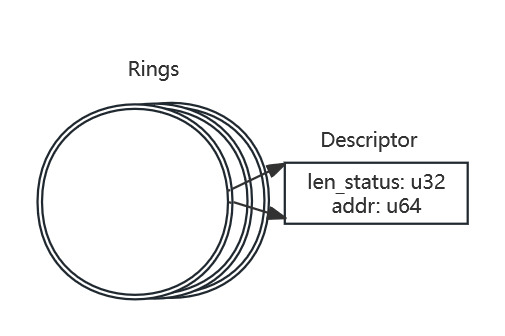
\includegraphics[scale=0.6]{./imgs/Rings_and_Descs.jpg}        
        \captionof{figure}{DMA 描述符与环}
    \end{minipage}
    \end{adjustwidth}

    \begin{lstlisting}[language=C
        , caption={Initialize Rx priority queues}
        , label={code::InitRxRings}
        , numbers = left
        , breaklines=true
        , breakatwhitespace=true]
static int bcmgenet_init_rx_ring(struct bcmgenet_priv *priv, unsigned int index, unsigned int size, unsigned int start_ptr, unsigned int end_ptr);
for (i = 0; i < priv->hw_params->rx_queues; i++) { // 初始化函数
    ret = bcmgenet_init_rx_ring(priv, i, priv->hw_params->rx_bds_per_q,
                    i * priv->hw_params->rx_bds_per_q, (i + 1) *
                    priv->hw_params->rx_bds_per_q);
    if (ret) return ret;
    ring_cfg |= (1 << i);
    dma_ctrl |= (1 << (i + DMA_RING_BUF_EN_SHIFT));
    \end{lstlisting}

    
    在具体实现层面其实没有什么特殊于前者的,基本上就是按照原先 cvitek 网卡驱动的开发过程进行的开发,
    同时,由于 BCM54213PE 的相关寄存器手册不对外进行开发,大部分的寄存器操作都是从 u-boot 或者 树莓派linux
    中进行的参考,只不过是根据 tock-registers 有界寄存器规约,将原本 u-boot 中存在的大量由
    宏或者裸地址进行声明的地址位置转变成为了 rust 语言下的定义,并且利用其边界检查等功能,进一步的
    保证了寄存器的操作的安全性,同时也提供了更加符合人体工学的寄存器操作\ref{tock_register}。

    \begin{lstlisting}[language=Rust
        , caption={tock register 包装}
        , label={code::tock_register}
        ]
        register_structs! {
            Channel {
                (0x00 => CS: ReadWrite<u32, CS::Register>),
                (0x04 => CONBLK: ReadWrite<u32, CONBLK::Register>),
                (0x08 => TI: ReadWrite<u32, TI::Register>),
                (0x0c => S_AD: ReadWrite<u32, S_AD::Register>),
                (0x10 => D_AD: ReadWrite<u32, D_AD::Register>),
                ...
            },
        } ...
        register_bitfields! { u32,
        CS [ // Control and Status registers
            RESET OFFSET(31) NUMBITS(1),
            ABORT OFFSET(30) NUMBITS(1),
            DISDEBUG OFFSET(29) NUMBITS(1),
            WAIT_FOR_OUTS_TANDING_WRITES OFFSET(28) NUMBITS(1),
            PANIC_PRIORITY OFFSET(20) NUMBITS(3),
            PRIORITY OFFSET(16) NUMBITS(4),
            ...
        ], CS_DMA4 [ ... ] ...}
    \end{lstlisting}

    在进行了大量的适配以及检查之后,在树莓派层面上成功完成了收发以太网数据帧的操作。

    \begin{figure}[ht]
        \centering
        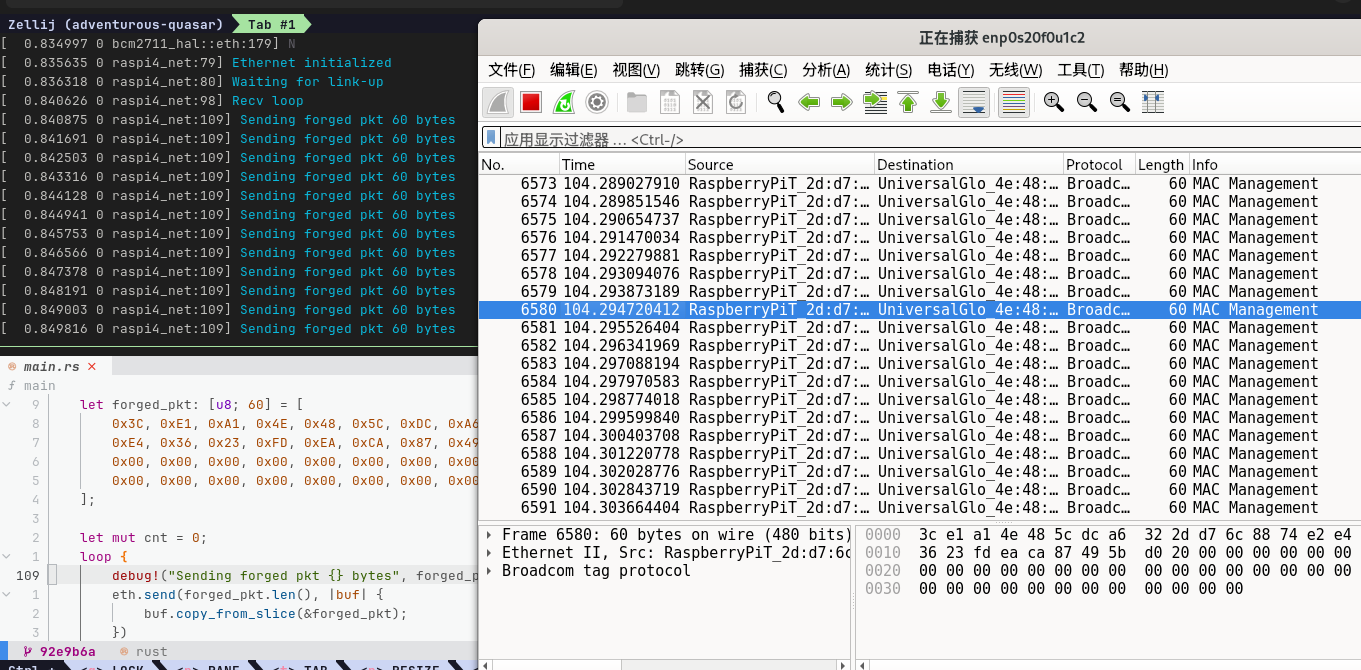
\includegraphics[scale=0.3]{./imgs/树莓派通信正常.jpg}
        \caption{树莓派通信正常}    \label{fig::树莓派通信正常}
    \end{figure}

    % TODO: 考虑添加图片说明这个过程



    % TODO: 后面看是用我自己的驱动还是直接用现成的

    \subsection{FPM383F 指纹识别模块串口通信单元分析}

    UART(Universal Asynchronous Receiver/Transmitter,通用异步收发传输器)也常被称为串口。
    UART 总线是在开发中使用频率最高的数据总线,其最大的特点就是在其上进行传输的时候仅需要三根信号线(Tx,RX,GND)
    就可以实现基本的信号传输功能而不需要常见同步传输所需要的时钟线。

    在这种异步收发传输器上,由于没有如同同步通信时所享有的时钟信号,需要以一种特殊的方式对于一个二进制信号的起始与终止进行规范,
    以方便进行读取的时候能够将信号线上进行传输的高低电平正确的转换成为二进制信号,UART 中要求通信双方均在其内部对于波特率进行设置
    且设置为相同值,就比如说当前指纹模块与树莓派主控模块之间采用的是57600Bps,就相当于在信号线上进行通信的时候,每个信号占据 1/57600 s。

    在信号线上没有进行传输的时候,信号线上保持高电平。在传输开始时,发送端会特地给一个低电平作为传输开始标记
    接受端收到了这个信号之后根据前面规定的每隔 (1/波特率) 秒对于信号线电平进行采样,将八个电平信号转换成为实际的字节数据。

    \begin{figure}[ht]
        \centering
        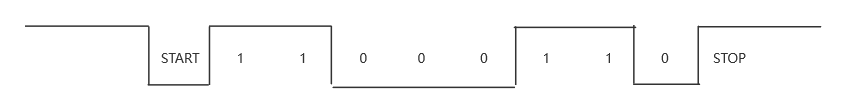
\includegraphics[scale=0.4]{imgs/UART跳变图.png}
        \caption{UART 跳变图}    \label{fig::uart}
    \end{figure}

    FPM383F 通信协议要求在串口层面使用小端序,十位帧格式(1位起始位,1位停止位,8位数据位),默认采用 57600Bps进行数据传输。
    \cite{noauthor_fpm383c_nodate}

    根据 FPM383F 通信协议的规定,串口层面传输的字节数据,在链路层面实际上以类似于下文中的数据结构\ref{FPM383F::UARTdataFrame}进行存在,
    在进行发送的时候逐个字节的进行传输。\cite{noauthor_fpm383c_nodate}
    从软件层面上讲,无论是发送还是由串口接收数据,均只需要对于对应 UART 的 DR 寄存器进行逐个字节读取或写入即可,具体内容被实现在硬件层面。
    
    \begin{table}[ht]
        \centering
        \begin{tabular}{|l|l|l|l|l|}
        \hline
        格式        & 帧头 & 应用层长度 & 帧头校验和 & 应用层数据 \\ \hline
        长度(bytes) & 8  & 2     & 1     & 7+N   \\ \hline
        \end{tabular}
        \caption{UART 数据帧格式表} \label{FPM383F::UARTdataFrame}
    \end{table}
    
    根据 FPM383F 通信协议的设定,应用层面其实由两种类型的命令构成。一种是主机向从机发送的请求,如图 \ref{FPM383F::UARTUserRequest}
    所示,另一种是从机(FPM383F)响应主机的请求,向主机发送响应,如图 \ref{FPM383F::UARTUserResponse}

    \begin{table}[ht]
        \centering
        \begin{tabular}{|l|l|l|l|l|}
        \hline
        \multicolumn{1}{|c|}{格式} & 校验密码 & 命令 & 数据内容        & 校验和 \\ \hline
        长度(Byte)                 & 4    & 2  & N(0$\sim$n) & 1   \\ \hline
        \end{tabular}
        \caption{UART 请求格式表} \label{FPM383F::UARTUserRequest}
    \end{table}

    \begin{table}[ht]
        \centering
        \begin{tabular}{|l|l|l|l|l|l|}
        \hline
        \multicolumn{1}{|c|}{格式} & 校验密码 & 命令 & 错误码 & 数据内容        & 校验和 \\ \hline
        长度(Byte)                 & 4    & 2  & 4   & N(0$\sim$n) & 1   \\ \hline
        \end{tabular}
        \caption{UART 响应格式表} \label{FPM383F::UARTUserResponse}
    \end{table}

    我这里采用我实现过程中相对比较复杂的一个部分,对于主从机响应的整个过程进行说明,如图\ref{FPM383F::DownloadFingerPrintInfo}所示。
    在我们从指纹模块获取对应指纹信息并且上传到上位机的时候,我们需要先使用0x53命令,向串口模块请求上传对应 ID 的指纹信息,
    指纹模块在没有出现错误的情况下会反馈特征长度,同时错误码置为0,出错的时候则反之。
    获取到该ID对应的整体特征长度之后,我们就可以通过循环命令,逐帧
    \footnote{根据通信手册,在同一帧下用户层最多只能添加128位的数据(在此处特指用于传输特征信号的信息位),因此需要逐帧进行发送}
    请求指纹模块上传该部分的指纹特征信息,最终在上位机将上述全部指纹特征信息整合到一起。

    \begin{figure}[H]
        \centering
        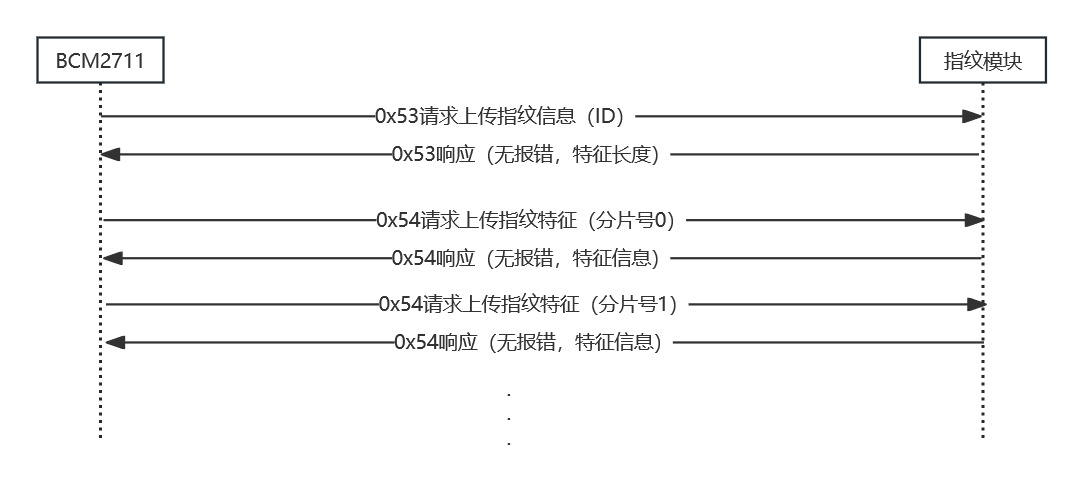
\includegraphics[scale=0.4]{./imgs/指纹信息下载.jpg}
        \caption{指纹信息下载}    \label{FPM383F::DownloadFingerPrintInfo}
    \end{figure}    

    \subsubsection{实现说明}

    在树莓派上提供了一系列与 UART 相关的寄存器,如 UART0, UART1(mini), 
    UART2-5等,考虑到目前 GPIO 口的占用情况,我选用了 GPIO4,5 所对应的串口
    UART3 来完成串口信息交换。

    我参照 2020 年 jonlamb-gh rpi4-rust-workspace 仓库\cite{rpi4-rust-workspace}
    提供的基于树莓派 UART 的串口树莓派初始化方案,进行了大量的适应性修改,在原先仅实现了串口收发包的基础上
    实现了对于 FPM383F 通信协议的适配,实现了解析,生成等功能。同时,由于根据上位机中实现指纹注册功能的设计,
    我同样使用 python 语言在上位机中实现了对应的功能
    \footnote{没有任何基于py语言的有关实现,唯一一个\href{micropython-HLK-FPM383C}{https://github.com/deerbleats/micropython-HLK-FPM383C}, 是在嵌入式设备上完成的处理工作}。

    具体算法抽象如下:

    \begin{algorithm}[H]
    \caption{以太网帧解析算法}
    \label{algorithm::UART}
    \begin{algorithmic}[1]
    \Function{parse}{$ser$} 
        \State $frame\_head \gets [0xF1, 0x1F, 0xE2, 0x2E, 0xB6, 0x6B, 0xA8, 0x8A]$ \Comment{帧头固定}
        \State $frame\_data \gets$ array of size 256 filled with 0 \Comment{考虑到全局分配,暂时采用数组}
        \State $len \gets 0$
        \State $cnt \gets 7$ \Comment{帧头的最后一个元素为7}
        \While{true}
            \State $data \gets$ read one byte from serial port $ser$ \Comment{逐字节读数据}
            \If{$frame\_data[0:8] \neq frame\_head[:])$}
                \State $frame\_data[0:8] \gets frame\_data[1:9]$
                \State $frame\_data[8] \gets 0$ \Comment{清理残余}
                \State $frame\_data[7] \gets data$
            \EndIf
            \If{$frame\_data[0:8] == frame\_head[:]$}
                \State $frame\_data[cnt] \gets data$
                \If{$cnt > 11$}
                    \State $len \gets$ convert bytes to integer($frame\_data[8:10]$)
                \EndIf
                \State $cnt \gets cnt + 1$
            \EndIf
            \If{$len \neq 0$ and $(cnt - 11) == len$} \Comment{确保当前帧的全部数据均已被收集}
                \State \Return $(len, frame\_data[11:cnt])$ 
                \Comment{这是一个简单抽象,对应到上/下位机有不同实现}
            \EndIf
        \EndWhile
    \EndFunction
    \end{algorithmic}
    \end{algorithm}
    
    考虑到实现的便捷程度,我并没有在下位机中实现对应帧的和校验,只是采用了简单的
    帧头循环方式,实现了对于串扰数据等因素导致的乱码使帧头校验不通过的情况进行了预防。
